\documentclass{article}
\usepackage{graphicx}
\usepackage{amsmath}
\usepackage{hyperref}
\usepackage[margin=1in]{geometry}

\title{Project I: Explainable AI for Image Classification using Twin System and Grad-CAM}
\author{Aryan Jain \\
INFO 692: Explainable AI \\
May 17, 2025}
\date{}

\begin{document}

\maketitle

\section{Introduction}
Explainable Artificial Intelligence (XAI) has become a critical area in understanding the behavior of machine learning models, particularly in sensitive or high-risk applications. In this project, I explored post-hoc XAI techniques applied to a binary image classification task: distinguishing between real and AI-generated (fake) cat images. My goal was not just to train a high-performing model, but also to make its decision-making process transparent.

I applied two complementary XAI methods:
\begin{itemize}
    \item \textbf{Grad-CAM (Gradient-weighted Class Activation Mapping)}: a technique that highlights important regions in an image that contribute most to the model's prediction~\cite{gradcam}.
    \item \textbf{Twin Case-Based Reasoning (Twin CBR)}: an approach that retrieves similar training examples based on learned embeddings, providing an example-based rationale~\cite{chen2018, barnett2021}.
\end{itemize}

\section{Dataset}
The dataset consisted of 300 cat images:
\begin{itemize}
    \item 150 real cat images collected from public online datasets
    \item 150 fake cat images generated using the diffusion model \texttt{google/ddpm-cat-256}~\cite{ddpm}
\end{itemize}

\textbf{Preprocessing:}
\begin{itemize}
    \item All images were resized to 224x224
    \item Normalized using CIFAR-style mean and std of 0.5
\end{itemize}

\textbf{Train/Validation Split:}
\begin{itemize}
    \item 200 images for training (100 real, 100 fake)
    \item 100 images for validation (50 real, 50 fake)
\end{itemize}

\section{Model}
I used a pretrained ResNet-18 model and fine-tuned it for binary classification by modifying the final fully-connected layer to output two classes: real and fake.

\subsection*{Training Configuration}
\begin{itemize}
    \item Optimizer: Adam (learning rate = $1 \times 10^{-4}$)
    \item Loss function: CrossEntropyLoss
    \item Epochs: 10
    \item Batch size: 32
\end{itemize}

The final model achieved \textbf{91\% accuracy} on the validation set.

\subsection*{Evaluation Metrics}
To assess model performance, I computed a confusion matrix and classification report:

\begin{figure}[h]
    \centering
    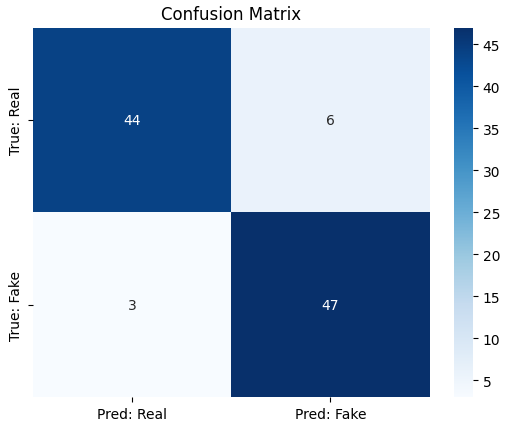
\includegraphics[width=0.6\linewidth]{img/confusion_matrix.png}
    \caption{Confusion Matrix and Classification Report}
\end{figure}

\begin{itemize}
    \item \textbf{Accuracy:} 91\%
    \item \textbf{Precision (Real):} 0.94 \quad \textbf{Recall (Real):} 0.88
    \item \textbf{Precision (Fake):} 0.89 \quad \textbf{Recall (Fake):} 0.94
    \item \textbf{F1-Score (Both Classes):} 0.91
\end{itemize}

\section{Experiments}

\subsection{Grad-CAM}
\textbf{Library:} \texttt{torchcam}~\cite{torchcam} \\
Activation maps were extracted from the final convolutional block (\texttt{layer4}). The resulting CAM overlays highlight areas of the image contributing most to the prediction.

\textbf{Visualizations:}
\begin{itemize}
    \item Original image
    \item Grad-CAM heatmap overlay
\end{itemize}

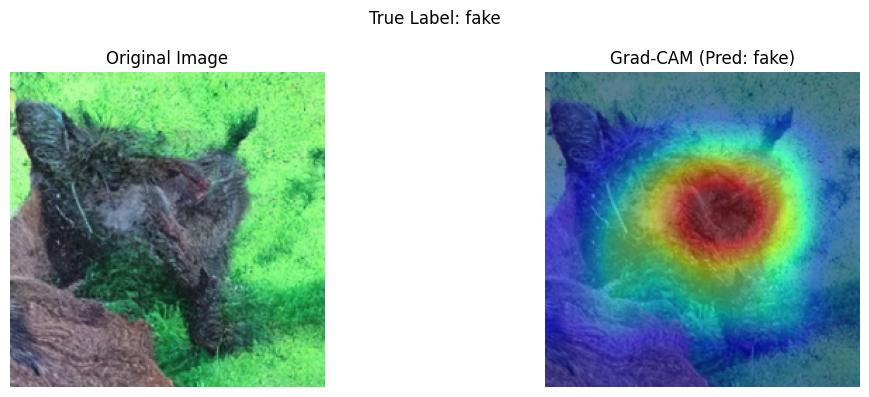
\includegraphics[width=0.9\linewidth]{img/sample_fake_0.png}\\
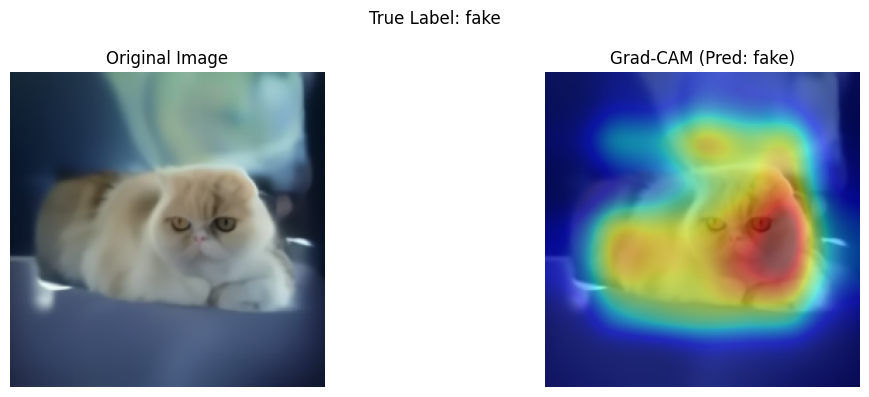
\includegraphics[width=0.9\linewidth]{img/sample_fake_1.png}\\
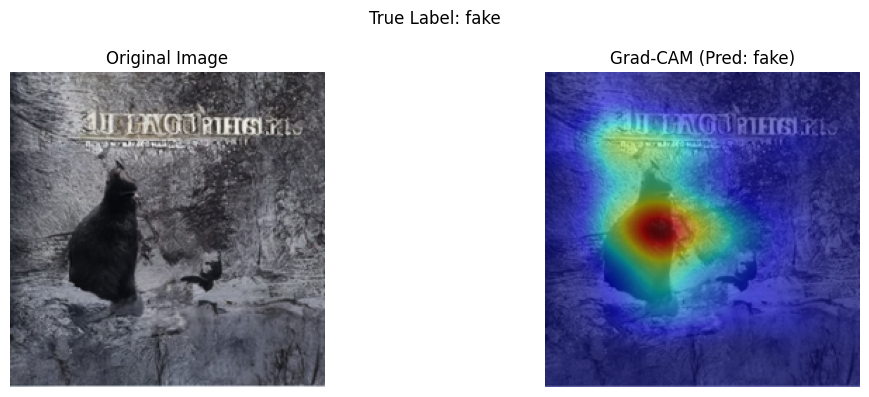
\includegraphics[width=0.9\linewidth]{img/sample_fake_2.png}\\
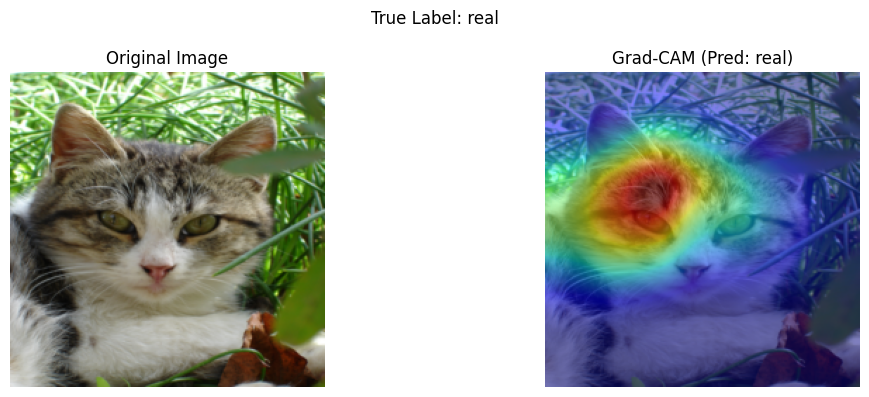
\includegraphics[width=0.9\linewidth]{img/sample_real_0.png}\\
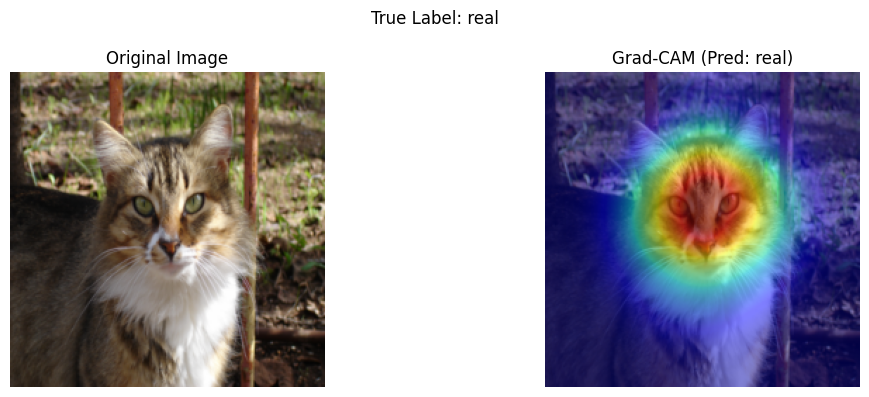
\includegraphics[width=0.9\linewidth]{img/sample_real_1.png}\\
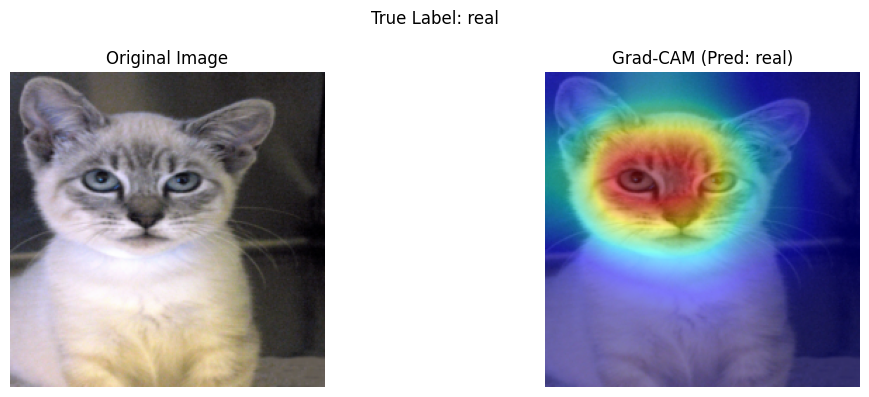
\includegraphics[width=0.9\linewidth]{img/sample_real_2.png}\\

\subsection{Twin CBR (Same-Class Neighbors)}
Feature vectors from the penultimate layer (\texttt{avgpool}) were used to compute cosine similarity.

\textbf{Steps:}
\begin{itemize}
    \item Extract embeddings for all training and validation images
    \item Identify $k=5$ nearest neighbors among training examples \textbf{with same predicted class}
    \item Retrieve neighbors for visual explanation
\end{itemize}

\textbf{Justification:} The model's decision is supported by visual similarity to known examples.\\

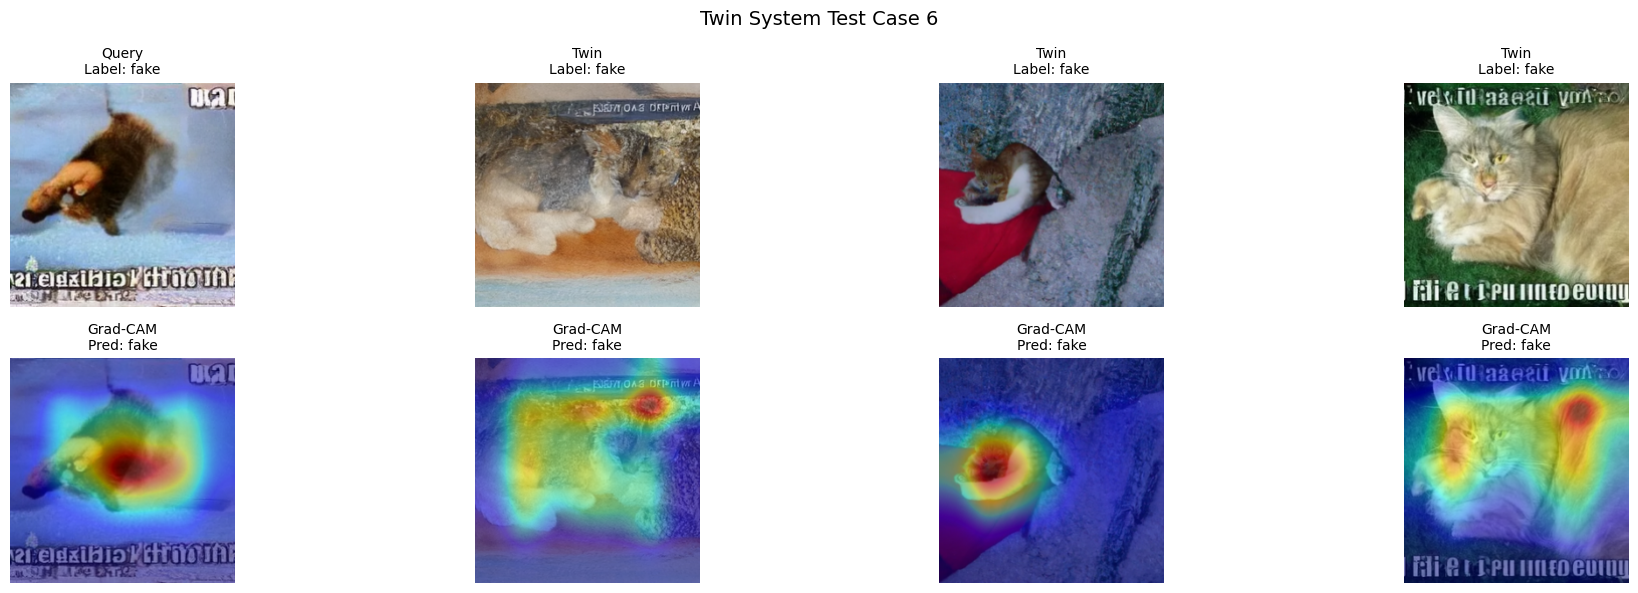
\includegraphics[width=0.9\linewidth]{img/twin_vis_test6.png}\\
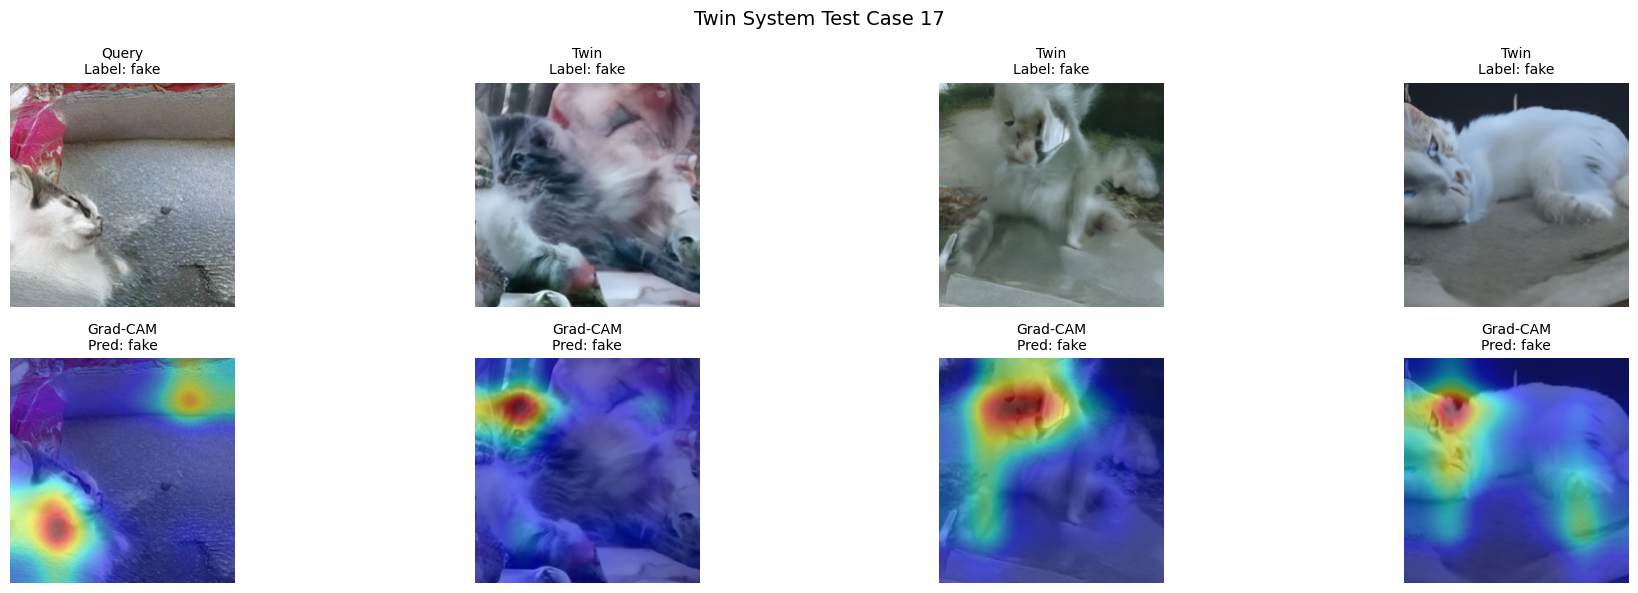
\includegraphics[width=0.9\linewidth]{img/twin_vis_test17.png}\\
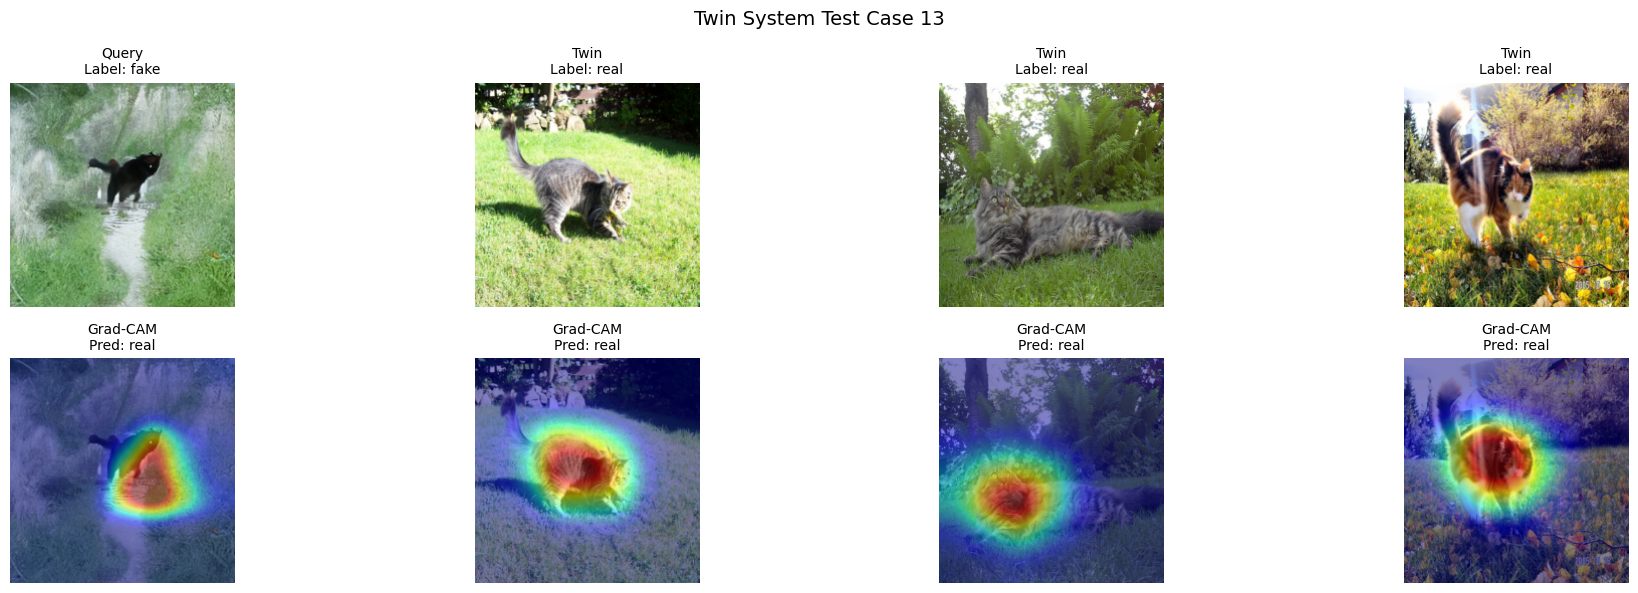
\includegraphics[width=0.9\linewidth]{img/twin_vis_test13.png}\\
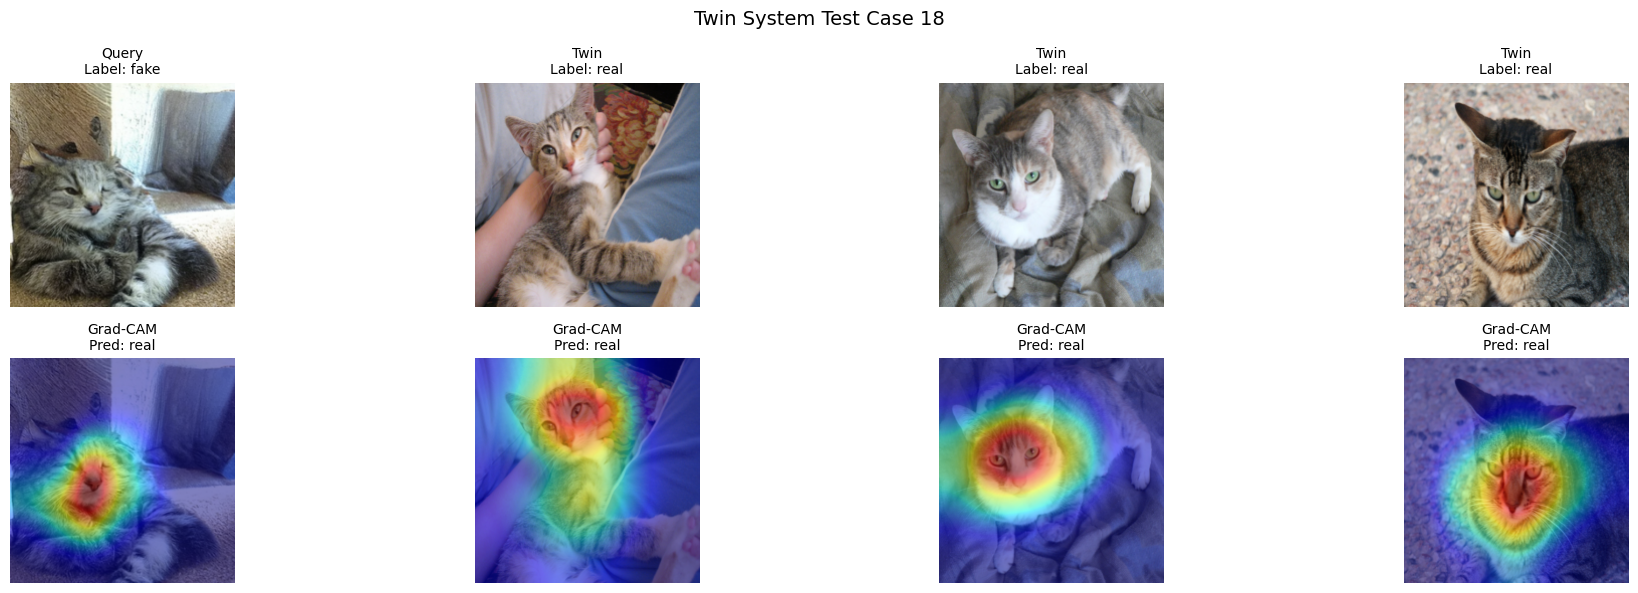
\includegraphics[width=0.9\linewidth]{img/twin_vis_test18.png}\\
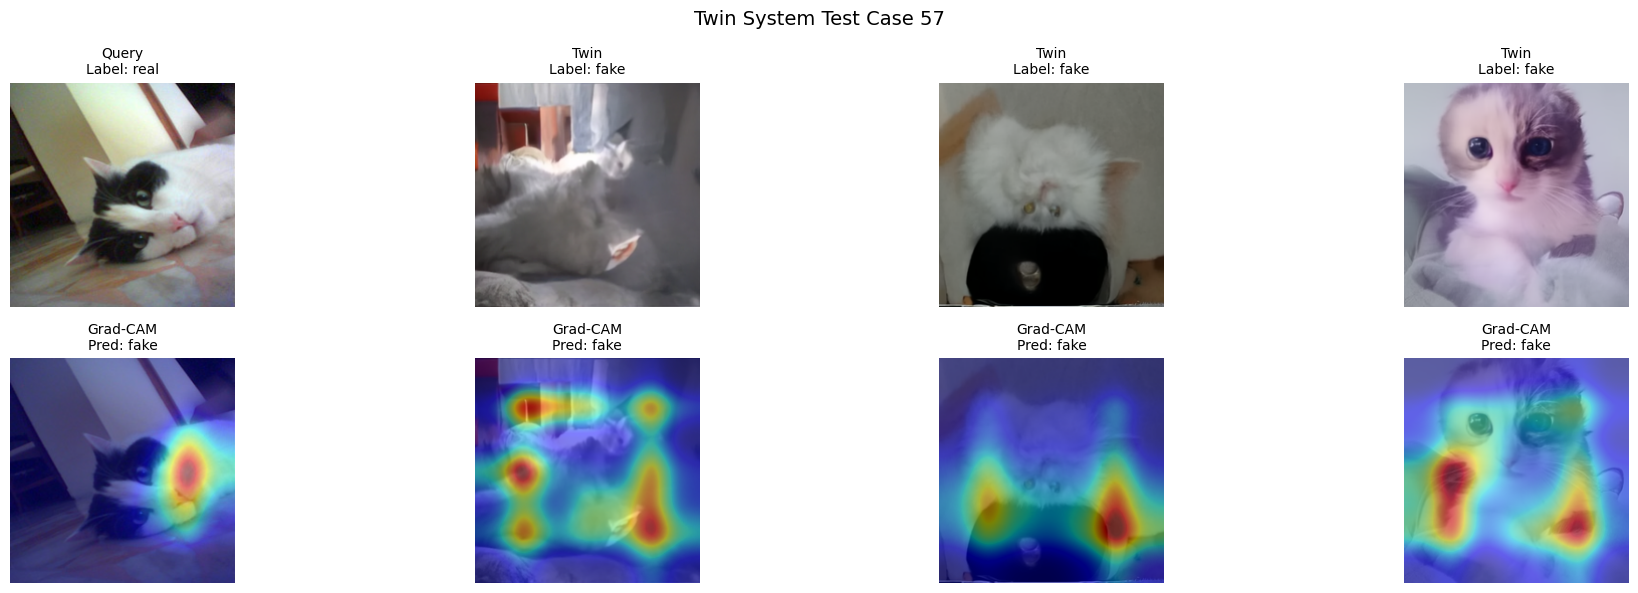
\includegraphics[width=0.9\linewidth]{img/twin_vis_test57.png}\\
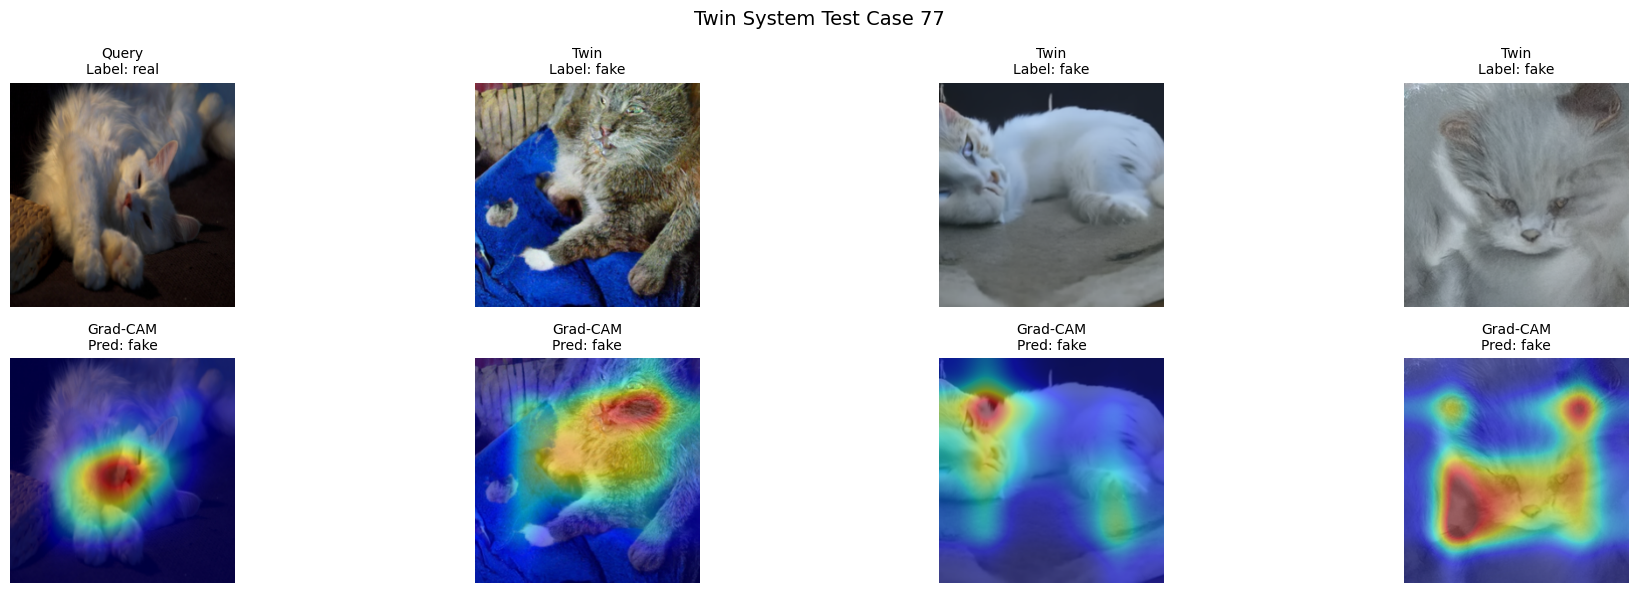
\includegraphics[width=0.9\linewidth]{img/twin_vis_test77.png}

\subsection{Misclassification Analysis}
I tracked test indices where the model:
\begin{itemize}
    \item Predicted "fake" for a real image : Test Cases [13, 18, 22, 34, 40, 44]
    \item Predicted "real" for a fake image  : Test Cases [57, 77, 80]
\end{itemize}

Twin panels and Grad-CAM overlays were used to interpret these misclassifications.

\section{Conclusion}
The combination of Grad-CAM and Twin System provided meaningful insights into the model's decision-making:
\begin{itemize}
    \item Grad-CAM highlights regions that triggered predictions
    \item Twin explanations give example-based rationales
\end{itemize}

This dual approach strengthens interpretability and fosters trust in AI image classifiers.

\section{Future Work}
\begin{itemize}
    \item Implement counterfactual examples (nearest neighbors from opposing class)
    \item Improve similarity search using CLIP embeddings
    \item Train a prototype-based network (ProtoPNet)
\end{itemize}

\subsection*{ProtoPNet Attempt}
I attempted to implement a ProtoPNet model using a ResNet-18 backbone with 10 prototypes per class. The architecture was designed to learn localized representations and classify images based on their similarity to learned prototypes. Although the implementation completed training, the performance was poor:

\begin{itemize}
    \item \textbf{Validation Accuracy:} 50\%
    \item \textbf{Class imbalance:} All samples predicted as real
\end{itemize}

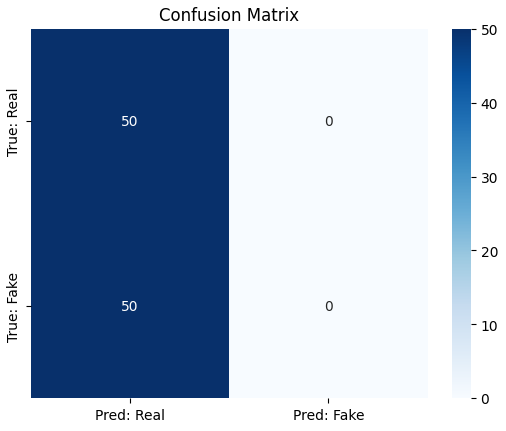
\includegraphics[width=0.6\linewidth]{img/protopnet_confmat.png}

Despite the low accuracy, I was able to visualize the learned prototypes:\\
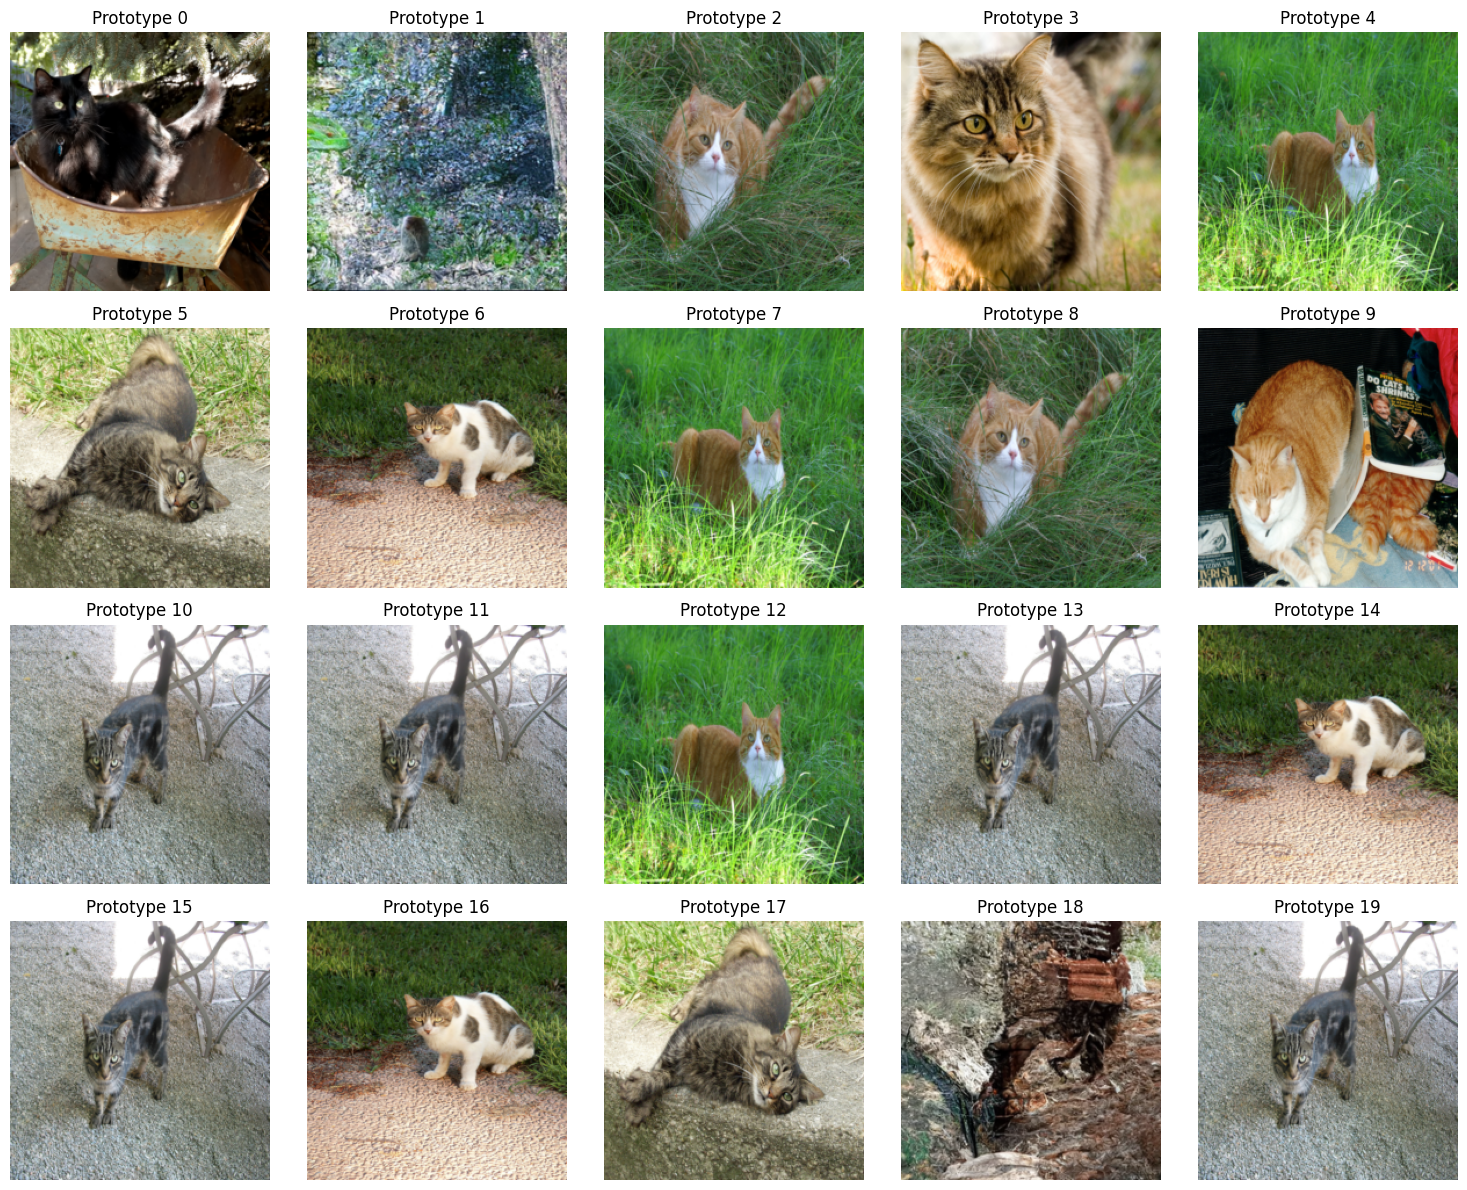
\includegraphics[width=0.9\linewidth]{img/protopnet_prototypes.png}\\



The model overfit to the "real" class and failed to activate relevant prototypes for fake images. I plan to revisit this architecture in future work by introducing regularization and prototype pruning.

\begin{thebibliography}{9}

\bibitem{gradcam}
Selvaraju, R.R., Cogswell, M., Das, A., Vedantam, R., Parikh, D., \& Batra, D. (2017).\\
\textit{Grad-CAM: Visual Explanations from Deep Networks via Gradient-Based Localization}.\\
Proceedings of the IEEE International Conference on Computer Vision (ICCV).

\bibitem{ddpm}
Ho, J., Jain, A., \& Abbeel, P. (2020).\\
\textit{Denoising Diffusion Probabilistic Models}.\\
Advances in Neural Information Processing Systems (NeurIPS).

\bibitem{torchcam}
TorchCAM Library, \url{https://frgfm.github.io/torch-cam/}

\bibitem{chen2018}
Chen, C., Li, O., Tao, C., Barnett, A. J., Su, J., \& Rudin, C. (2018).\\
\textit{This Looks Like That: Deep Learning for Interpretable Image Recognition}.\\
arXiv preprint arXiv:1806.10574.

\bibitem{barnett2021}
Barnett, A. J., Schwartz, F. R., Tao, C., Chen, C., Ren, Y., Lo, J. Y., \& Rudin, C. (2021).\\
\textit{A Case-Based Interpretable Deep Learning Model for Classification of Mass Lesions in Digital Mammography}.\\
Nature Machine Intelligence, 3(12), 1061--1070.

\end{thebibliography}

\end{document}
